\documentclass[11pt]{article}
\usepackage{geometry}
\geometry{a4paper, total={6in, 8in}, margin={0in}}
\usepackage{wrapfig}
\usepackage{graphicx}
\usepackage{fullpage}
\usepackage{listings}
\usepackage{xcolor}
\usepackage{listings}
\usepackage{xparse}

\NewDocumentCommand{\codeword}{v}{%
\texttt{\textcolor{darkgray}{#1}}%
}

\lstset{language=C,keywordstyle={\bfseries \color{blue}}}


\begin{document}

\title{C Project Final Checkpoint}
\author{Kareem Mehanna, Faraz Malik, Belal Makhzoum, Mohamed Sharif}
\date{June 23, 2023}

\maketitle

\section{Assembler}
Our implementation of {\it assembler} was quite similar to the {\it emulator}. Given that both similarly decode and identify instructions, it seemed prudent to ensure the {\it assembler} followed a structure parallel to that of  {\it emulator}, resulting in ease of development with a familiarised structure. 

\subsection{Structure}
The decomposition of “assembler” is as follows:
\begin{itemize}
\item File
    \begin{itemize}
    \item Read assembly source
    \item Write machine output
    \end{itemize}
\item Heap-allocated memory (read/write)
\item Instruction
    \begin{itemize}
    \item Opcode identification
    \item Encoding (branch, data processing, single data transfer)
    \end{itemize}
\end{itemize}

It is worth noting that the breakdown is highly similar to the {\it emulator}, allowing the control flow in the central function to remain near-identical. We recognised earlier that the heap-allocated \codeword{array} representation of program memory would be used to store the encoded assembly instructions during the {\it assembler}'s iteration. This resulted in the complete reuse of this critical data structure, saving development time.

\subsection{Implementation}
The {\it assembler} reads, normalises and splits assembly lines into their corresponding opcodes and operands. The instructions are then encoded to machine code based on their respective instruction types. The machine code would be stored in {\it little-endian} format in the heap-allocated memory. After encoding the instructions, the data in memory would be written to the binary output file.

We constructed many utility functions, which followed the {\it assembler} pipeline closely. The program loaded assembly instructions, then performed an implementation of the two-pass {\it assembler}: 
\begin{enumerate}
    \item The first pass created a symbol table that associated labels with memory addresses, stored as an \codeword{array} of heap-allocated \codeword{struct}s.
    \item The second pass encoded assembly instructions to their binary equivalent, as per the specification's guidelines. The resulting \codeword{uint32_t} was stored in {\it little-endian} format in the heap-allocated memory.
\end{enumerate}

The opcode directed the selection of the appropriate {\it assembler} sub-function, i.e. assembleBranch, assembleDataProcessing, etc. that would return the binary instruction encoded as a \codeword{uint32_t}.

\section{Extension - {\it sunriseIDE}}
Our extension involved the natural combination of the {\it assembler} and compiler, with the added functionality of comprehensive syntax analysis, into a terminal-based development tool, coined {\it sunriseIDE}. The meaningful processing is the syntax analysis, which would provide bespoke error messages for each instruction type, with the implementation of the \codeword{<regex.h>} package. Also, flagging any references to undeclared labels against a label map on valid assembly code.

\subsection{Structure}
The decomposition of {\it sunriseIDE} is as follows:

\begin{itemize}
\item Syntax analysis
    \begin{itemize}
        \item Line pattern matching
        \item Label verification
    \end{itemize}
\item Pipelining
    \begin{itemize}
        \item Compile (analyse → assemble)
        \item Run (Compile → emulate[run])
        \item Run (Compile → emulate[debug])
    \end{itemize}
\end{itemize}

\begin{figure}[h]
  \centering
  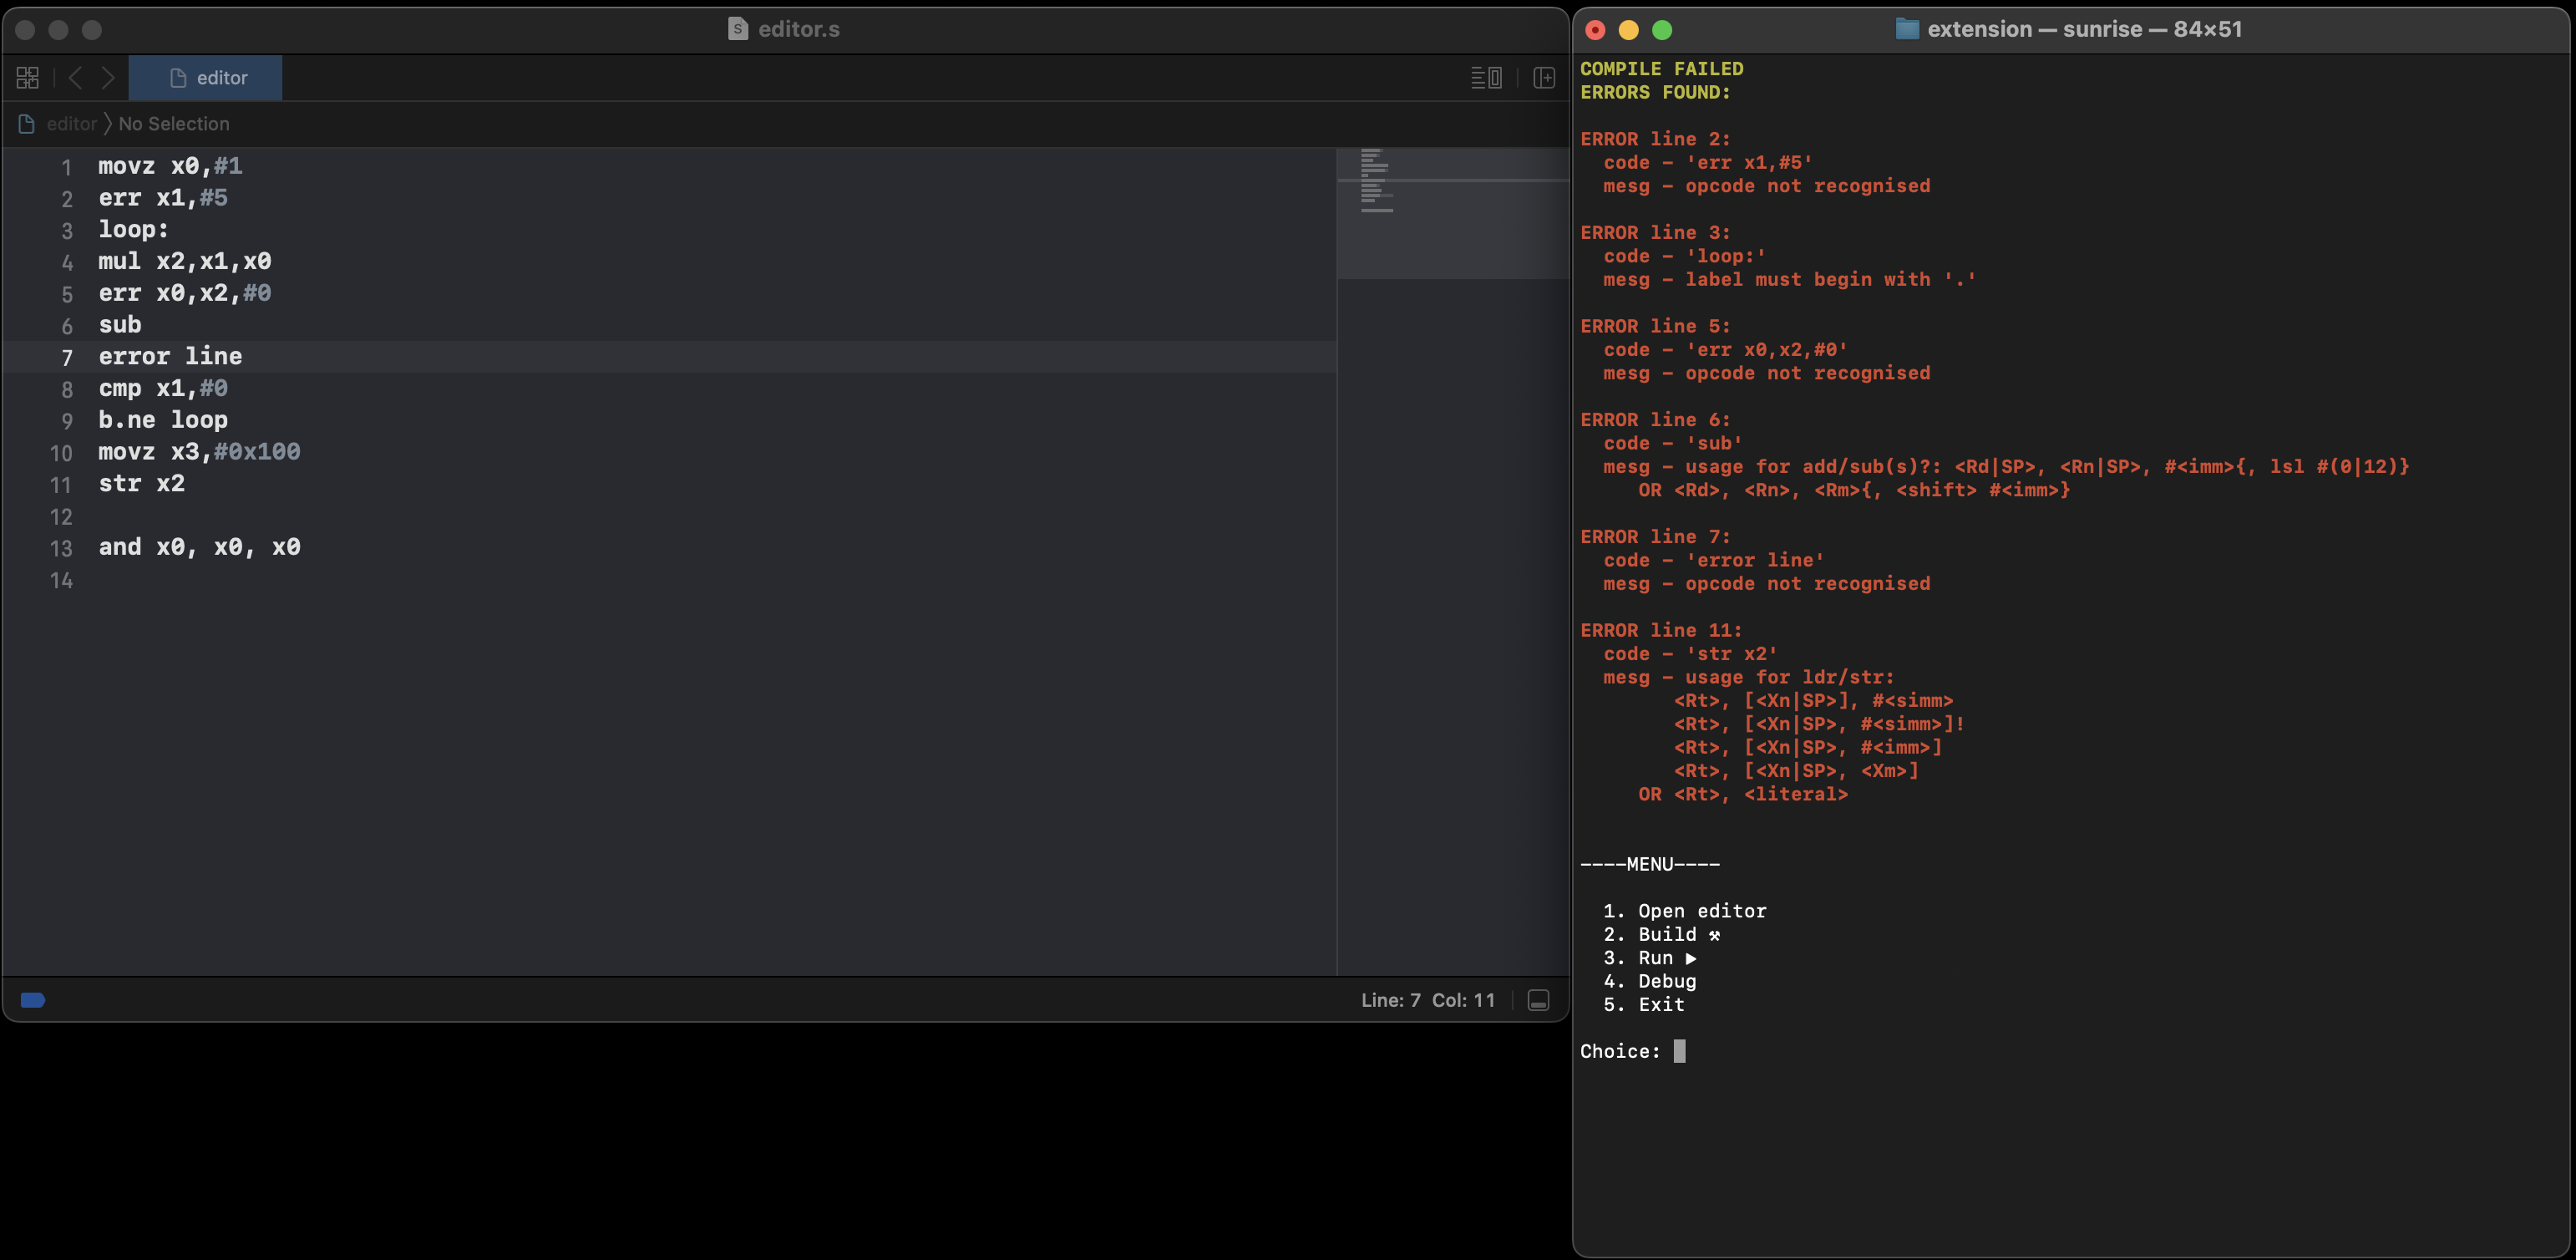
\includegraphics[scale=0.9,width=14cm]{example_use.png}
  \caption{Example usage with erroneous assembly lines being pattern-matched against the formats outlined in p.24 of the specification.}
\end{figure}

\newpage
\subsection{Implementation}
The {\it sunriseIDE} allows the user to open the \codeword{editor.s} from its interface (via integrated terminal commands). When the user selects any menu option, the file is verified with the syntax analyser, and is placed into a string \codeword{array}. Based on user selection, the \codeword{array} is assembled and/or emulated.
There are two ways the assembly \codeword{array} is emulated:
\begin{itemize}
    \item Run
    
    Emulates through the code until the \codeword{and x0,x0,x0} instruction is encountered, and outputs the state of the program (registers and non-zero memory).
    \item Debug
    
    Outputs the state of the program after every single line is executed, allowing the user to control the step through the execution with a telling analysis.
\end{itemize}

\begin{figure}[h]
  \centering
  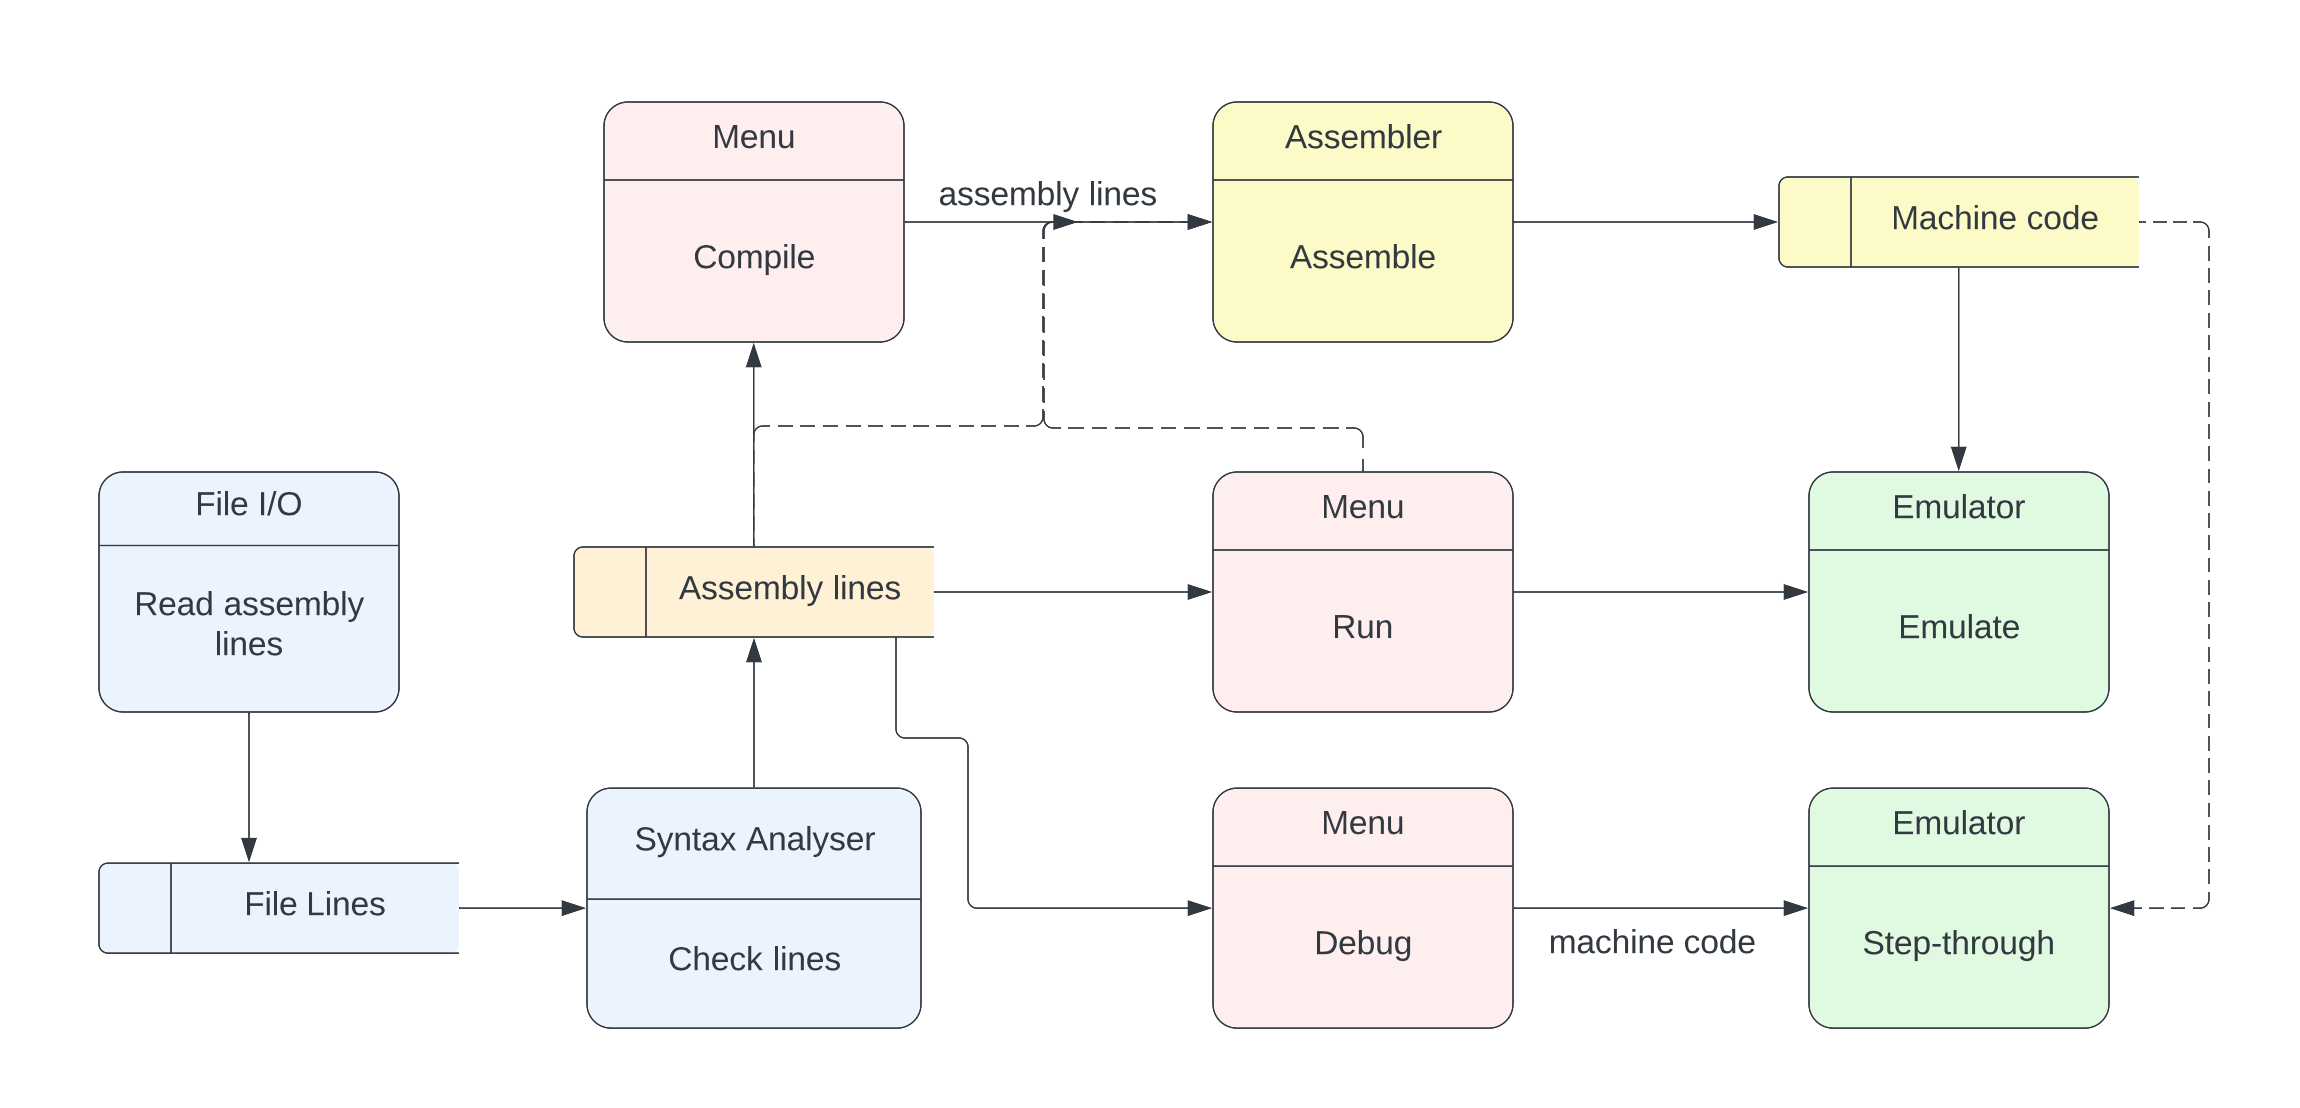
\includegraphics[scale=0.9,width=14cm]{data_flow.png}
  \caption{Data flow diagram highlighting key components of {\it sunriseIDE}, including the critical role of the syntax analyser in the pipeline.}
\end{figure}

\subsection{Challenges during implementation}
The {\it sunriseIDE} provided syntax analysis via regular expressions (regex) to match the littany of assembly line patterns (outlined in p.24 of the specification). We were faced with a choice here - either create a general pattern for all instructions, or to match every single row. The advantage of the latter would be providing more specific information on why the assembly line was rejected. The challenge was writing the regex in a manner that would ensure it minimise repetition, which was done by breaking down the regex into repeating components, such as keys, optional shifts, etc. This was charted territory, as it mirrored our encoding style for the {\it assembler}.

Given the {\it sunriseIDE} integrated both the assembler and emulator into its pipeline, we had resorted to interfacing with the executables directly for each. This was a temporary solution, only during the initial development stages. Later on, we had to resolve multi-directory dependencies for the \codeword{Makefile}, in order that the {\it sunriseIDE} executable would not also require the presence of other, separate executables.

\subsection{Testing}
The prerequisite of the {\it sunriseIDE} is that the {\it assembler} and {\it emulator} are error-free. The testing centred on three areas of functionality:
\begin{itemize}
    \item Correct integration of the {\it assembler} and {\it emulator}

    We had to modify the interfaces of the {\it assembler} and {\it emulator} to ensure it matched the requirements of the {\it sunriseIDE}. This required testing to ensure their usage behaved as expected.
    \item Regex patterns recognising assembly instructions

    We made use of incremental testing as we wrote the regex patterns to ensure we didn't overburden ourselves by accumulating this for the end.
    \item Recognising references to undeclared labels

    We tested this by confirming the label map added all labels, and the branch literal was correctly isolated. We also ensured the \codeword{labelContainsMap} function was correctly implemented.
\end{itemize}

Given the self-contained nature of assembly code, we believe our testing strategy to be fairly effective at ensuring syntax validation is functioning as expected. Also, we can rely on label map working, as we reused it from the {\it assembler}, which passed all tests.

Had we more time, we could implement certain logic checks to warn the user of potential problems, for example registers compared before a branch never being updated, or warnings for labels that were never used.

\section{Raspberry Pi}
\subsection{Implementation}
The code for part 3 was written in assembly, then assembled using our assembler and run on the Raspberry Pi. Our implementation wrote the buffer to a specific memory address each time the LED was required to turn on or off, mitigating the issue where the response would overwrite the existing buffer. Labels were used very frequently to allow for loops and to create "functions" which could be called multiple times. The frequency of the blinking can be changed very easily by changing the value stored in one register.
\subsection{Potential improvements}
Although the spec stated that only the LED on/off tag parameters would be overwritten by the buffer, we had to write the whole buffer each time. Ideally we would only write the overwritten parameters to improve efficiency, but we could not find a way to achieve this during the deadline. Debugging the program was also very difficult, even when using an emulator, but we could not find a better way to check the results without copying the assembled file into the SD card and running it every time. 


\pagebreak
\section{Reflections}
\subsection{Group reflection}
For the majority of our project we always tried to work in-person as much as we could. We worked side by side in the same room which allowed us to collaborate easier and prevent any misalignment that might have occurred. We could easily correct any doubts and we could easily monitor each other's work to allow us to judge whether we were working towards our goal. 

Our programming style was structured such that it was consistent throughout the project and each group member was aware of his responsibilities and tasks. We utilized an extension in Jetbrains Clion called CodeWithMe that allowed us to share our coding environment, which made it easy for everyone to review and modify pieces of code, as well as being extremely effective when debugging errors. We were able to pair program using this software and this greatly enhanced our productivity as well as eliminated the need for constant code sharing and merging branches. Even though we created different branches for different sections of code, we decided using CodeWithMe for smaller changes and for debugging allowed for a more seamless and efficient workflow.

During the development of the emulator we realized we had left a huge chunk of testing and debugging to the end of the timeline. For this reason we had to spend a whole day debugging errors to pass tests and we spent the previous 5 days developing the emulator. After learning from our mistakes from the emulator, we decided for the {\it assembler} we were to debug as we develop and take on an even more modular approach, and so we were able to isolate errors and detect why do we occur and in which function they would occur in. We significantly reduced our debugging time and spent 4 days developing and debugging the emulator. 

After completing the emulator and {\it assembler}, we branched off into two groups: one tackling the extension and one to program the Raspberry Pi. We were able to complete both in a reasonable amount of time, to prepare for the deadline.
\subsection{Individual reflections}
\subsubsection*{Kareem Mehanna}
Overall, the project went very well, with only minor hiccups along the way. The biggest contributing factor to this was meeting in person every day. This allowed problems to be discussed more easily and debugging was made much easier. This was the most important thing I would like to take forward when working on other projects with other groups in the future. Other beneficial techniques to carry forward include using project management software to divide up tasks, and performing incremental tests on individual functions rather than leaving all the tests to the end. This was a mistake that we made during the development of the emulator, but we made sure to correct it for the {\it assembler}. 

Before starting the project, I was concerned that organisation and deadlines would be much harder to manager in a group than if the project was individual. This did not turn out to be the case. Instead, our deadlines were simple to manage and very clear, enabling the smooth progress of the project. Every member of the group pulled their weight and did what was required of them, reducing the amount of work each person had to do.

\subsubsection*{Belal Makhzoum}
Due to the the various assisting softwares, development on the project went mostly smoothly. The consistent turn up of every group member daily made me along with all the other group members allowed be to be an asset to the group. I think that using group members functions easy as I understood at all time what everyone was doing and how the tasks were assigned. However, because I didn't test all of my parts in emulate during development, debugging at the end was slowed by one of my functions. However, I learnt from this and made sure to test during the {\it assembler} avoiding any problems being caused by my parts. I thought that adapting my coding style to match with my group and making my code understandable would be a weakness, however, I was able to adapt quickly to my group members and changing this coding style was not difficult. This was also partly due to the amount of communication that we had between each other.

Moreover, the positive group mindset and strong work ethic, made the group well ahead of schedule, making the entire project very stress free. This was also something that I thought would cause me to struggle with this project. 

\subsubsection*{Faraz Malik}
For this project, I felt very comfortable taking on a leading role. This involved taking the responsibility of breaking down each of the sections into individual, self contained tasks, which I then delegated to myself and the team. I ensured the distribution ensured no single person was overburdened, and kept the project on track for the deadline. As a result, we completed the emulator in the first week (w/c 29 May) and the assembler before the end of the second (w/c 5 June). 
We were able to incorporate revision for the C exam, which had a higher weighting than the project, seamlessly into our well-managed timeline. Therefore the project didn’t impede our ability to also carry on with other tasks. 

When entering the third (w/c 12 June), I made the judgement call to split the group into pairs. One was responsible for ensuring the Raspberry Pi was correctly set up, and the second for the extension. Thus we were able to complete the project by Monday, 19 June, and could focus attention on administrative tasks such as the write-up and planning the presentation video. 

Another help was the pre-existing relationship I had with my team members, which made it far more acceptable to set expectations (such as being in-person) and make requests (such as debugging emulator on a Saturday remotely). 


\subsubsection*{Mohamed Sharif}
I really enjoyed working with this group and found it to be one of the reasons for my growth. I collaborated well with them and discovered pair programming was a really excellent way to work on a project. Initially, I thought I was better at working solely independently but when working with your peers on a project with similar abilities, I learnt that we can complete a project way more effectively than if it was by myself. The diverse skill sets of my group members allowed me to gain new insights to a problem and and alternative way to solve it and they also compensated for my weaknesses. We worked in-person which allowed us to work together easier as we were in the same room but although this is sustainable for smaller and more intense projects, for larger projects it would be more sustainable for us to work online. 

Therefore, for next steps we would like to start working online and learn the best ways and tools to work online together. My group maintained a very warm and respectful attitude towards each other and I always felt my contributions and suggestions were not only heard but also critiqued for the betterment of the project.

Overall I am grateful for my team members for providing this valuable experience that contributed to both my professional and technical growth. I will carry these lessons forward to future group projects and improve on my weaknesses that previously held me back.

\end{document}
